% !TeX encoding = UTF-8
% !TeX root = master.tex
% !TeX spellcheck = en_US

\documentclass[xcolor=x11names,compress]{beamer}

%---------------------------------------------------------------------------------------------------
% Beamer configuration
%---------------------------------------------------------------------------------------------------

\setbeamertemplate{footline}[page number]{}
\setbeamertemplate{navigation symbols}{}
\setbeamertemplate{caption}[numbered]

\useoutertheme[subsection=false,shadow]{miniframes}
\useinnertheme{default}
\usefonttheme{serif}

\setbeamerfont{title like}{shape=\scshape}
\setbeamerfont{frametitle}{shape=\scshape}

\setbeamercolor*{lower separation line head}{bg=DeepSkyBlue4}
\setbeamercolor*{normal text}{fg=black,bg=white}
\setbeamercolor*{alerted text}{fg=red}
\setbeamercolor*{example text}{fg=black}
\setbeamercolor*{structure}{fg=black}

\setbeamercolor*{palette tertiary}{fg=black,bg=black!10}
\setbeamercolor*{palette quaternary}{fg=black,bg=black!10}

\renewcommand{\(}{\begin{columns}}
\renewcommand{\)}{\end{columns}}
\newcommand{\<}[1]{\begin{column}{#1}}
	\renewcommand{\>}{\end{column}}



%---------------------------------------------------------------------------------------------------
% Packages
%---------------------------------------------------------------------------------------------------

\usepackage{mathpazo}
\usepackage[utf8]{inputenc}
\usepackage[T1]{fontenc}
\usepackage[english]{babel}
\selectlanguage{english}
\usepackage{graphicx}
\usepackage{grffile}
\graphicspath{{figures/}}
\usepackage{float}
\usepackage{booktabs}
\usepackage{tabu}
\usepackage{rotating}
\usepackage{array}
\usepackage{multirow}
\usepackage{url}
\usepackage{hyperref}
\usepackage[capitalise,noabbrev,nameinlink]{cleveref}
\usepackage[nonumberlist,acronym,nomain,nowarn]{glossaries}
\usepackage[gen]{eurosym}
\usepackage{etoolbox}
\usepackage[center]{caption}
\glsdisablehyper
\makeglossaries

\makeatletter
\g@addto@macro{\UrlBreaks}{\UrlOrds}
\makeatother

%\overfullrule=3mm

%\newacronym{latex-label}{acronym}{acronym description}



%---------------------------------------------------------------------------------------------------
% Top matter
%---------------------------------------------------------------------------------------------------

\title{Recognition of Banknotes in Multiple Perspectives Using Selective Feature Matching and Shape Analysis}
\author{Carlos M. Costa\texorpdfstring{\\{\ttfamily carlos.costa@fe.up.pt}}{}}
\institute{Faculty of Engineering\\University of Porto\\Portugal}
\date{February 3, 2016\\{\small 11\textsuperscript{th} Doctoral Symposium in Informatics Engineering}}

\begin{document}

\begin{frame}
	\titlepage
\end{frame}



%---------------------------------------------------------------------------------------------------
% Outline
%---------------------------------------------------------------------------------------------------

\begin{frame}{Presentation Outline}
	\tableofcontents
\end{frame}



%---------------------------------------------------------------------------------------------------
% Sections
%---------------------------------------------------------------------------------------------------

\section{\scshape Introduction}\label{sec:introduction}

\subsection{Context}
\begin{frame}{Context}
	\begin{itemize}
		\item Most of commercial transactions are still done using physical currencies
		\item Most currencies banknotes were not designed to be usable by visually impaired people
		\item Detection of counterfeit banknotes could improve the reliability of ATMs and counting machines
		\begin{itemize}
			\item Ensure proper maintenance operations
			\item Confirm value and authenticity of banknotes
		\end{itemize}
	\end{itemize}
\end{frame}


\subsection{Objectives}
\begin{frame}{Objectives}
	Implementation of a generic banknote recognition system capable of recognizing banknotes with:
	\begin{itemize}
		\item Partial occlusions
		\item Folding
		\item Wrinkles
		\item Damage
		\item Multiple perspective views
		\item Multiple scales
		\item Environment clutter
		\item Several banknotes in same image
	\end{itemize}
\end{frame}

\section{\scshape Recognition System}\label{sec:methodology}

\subsection{Recognition System Overview}
\begin{frame}{Recognition System Overview}
	\begin{figure}
		\centering
		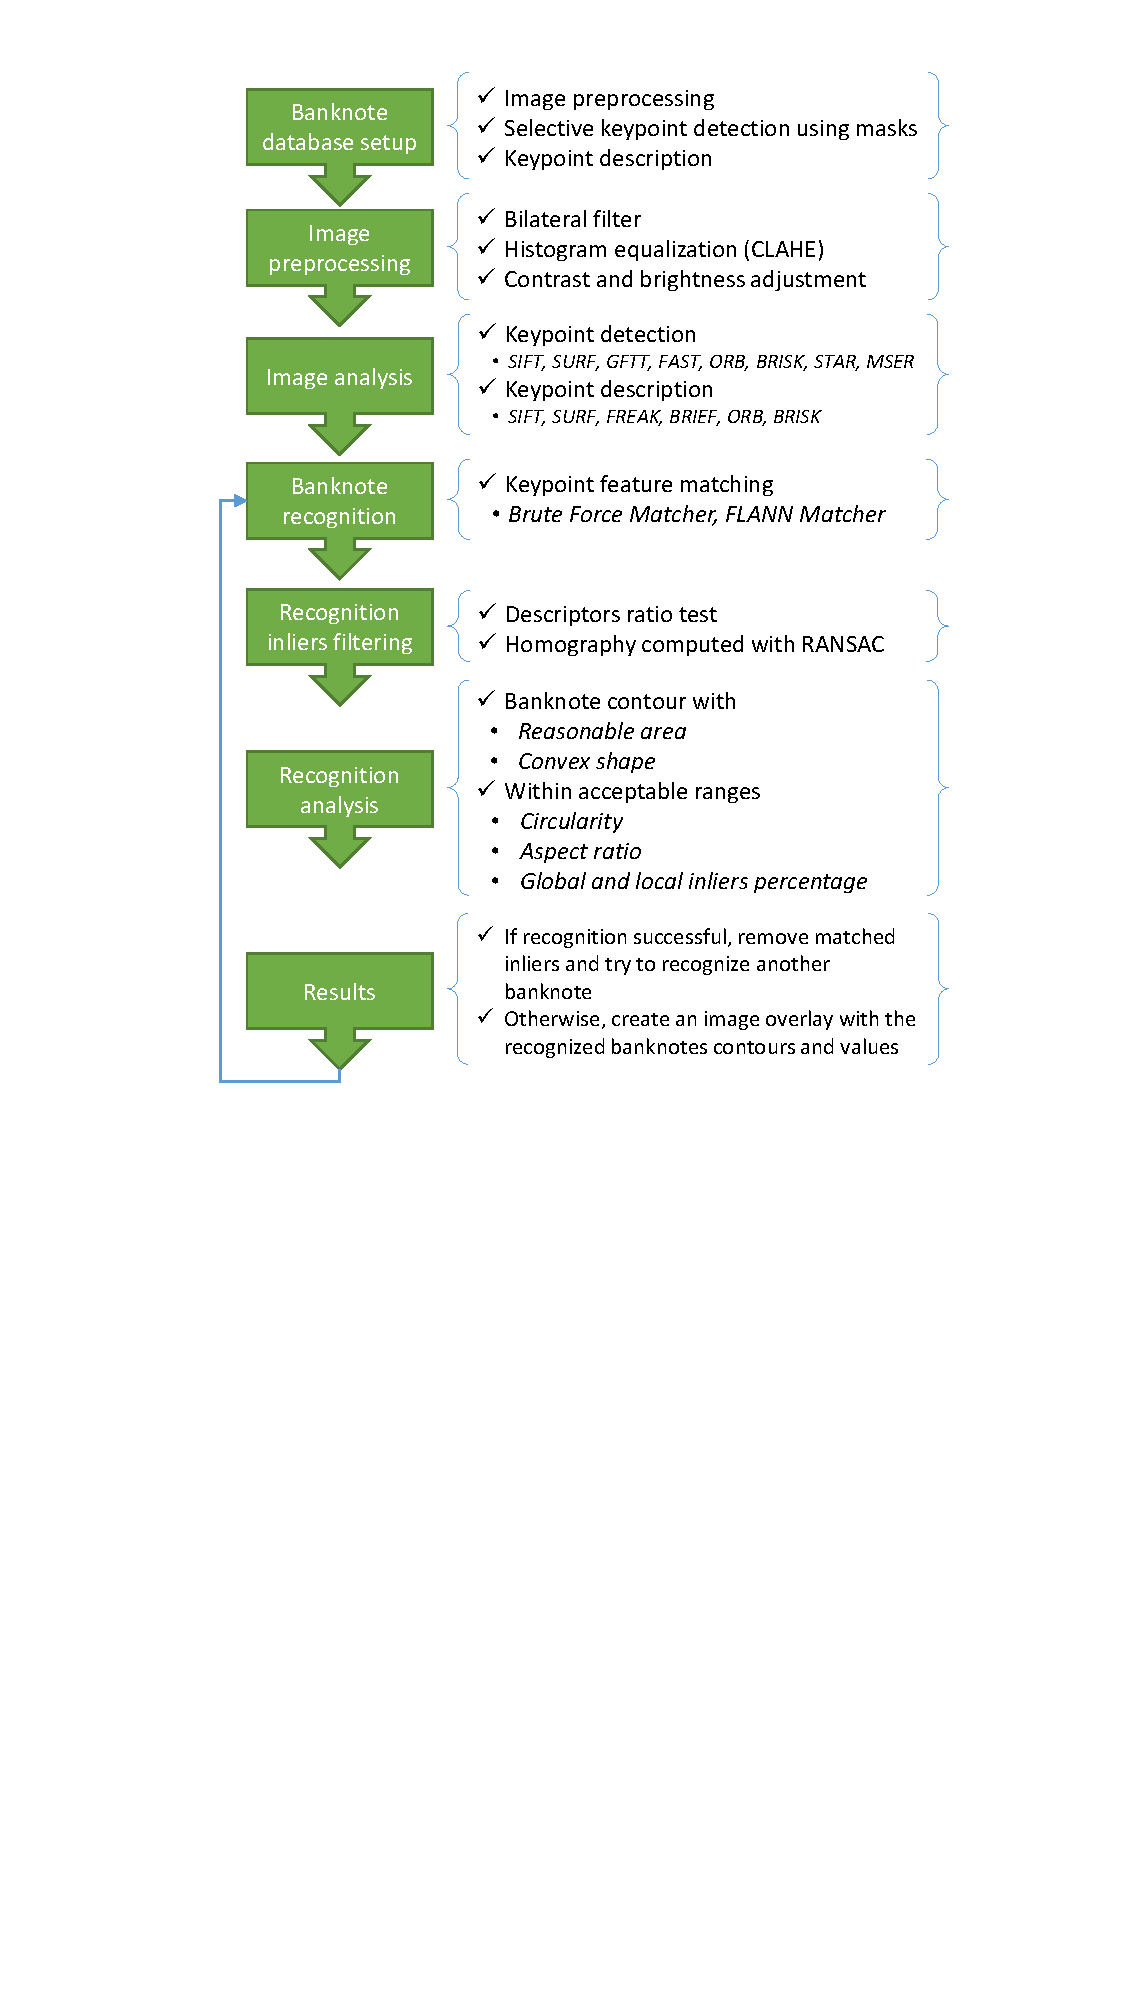
\includegraphics[width=0.45\linewidth]{system-overview}
		\label{fig:system-overview}
	\end{figure}
\end{frame}


\subsection{Banknote Database Setup}
\begin{frame}{Banknote Database Setup}
	\begin{itemize}
		\item Multi-resolution recognition database
		\begin{itemize}
			\item Image width of 256, 512 and 1024 pixels
		\end{itemize}
		
		\item Each banknote is subjected to
		\begin{itemize}
			\item Image preprocessing
			\item Selective keypoint detection using masks
			\item Keypoint description
		\end{itemize}
	\end{itemize}
	
	\begin{figure}[H]
		\centering
		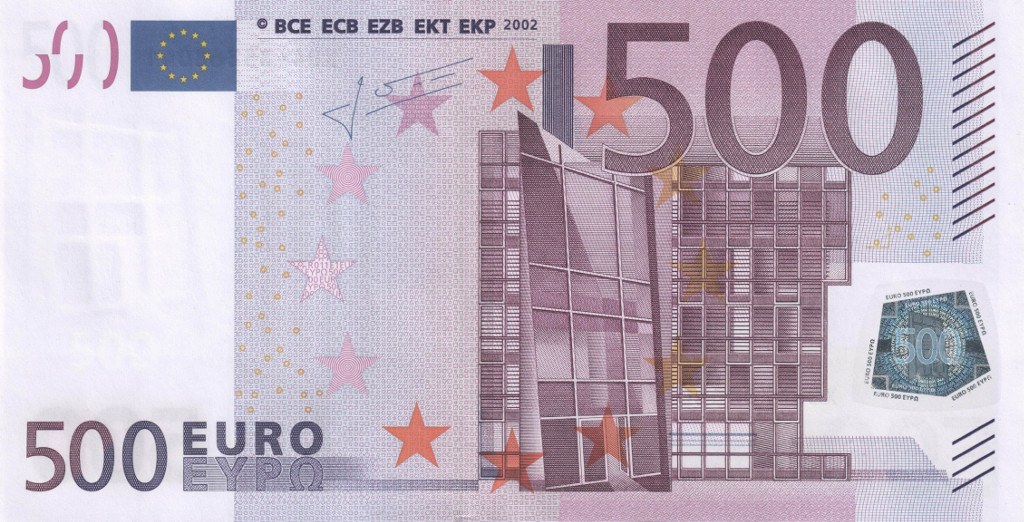
\includegraphics[width=.33\textwidth]{notes-masks/500eu-front}
		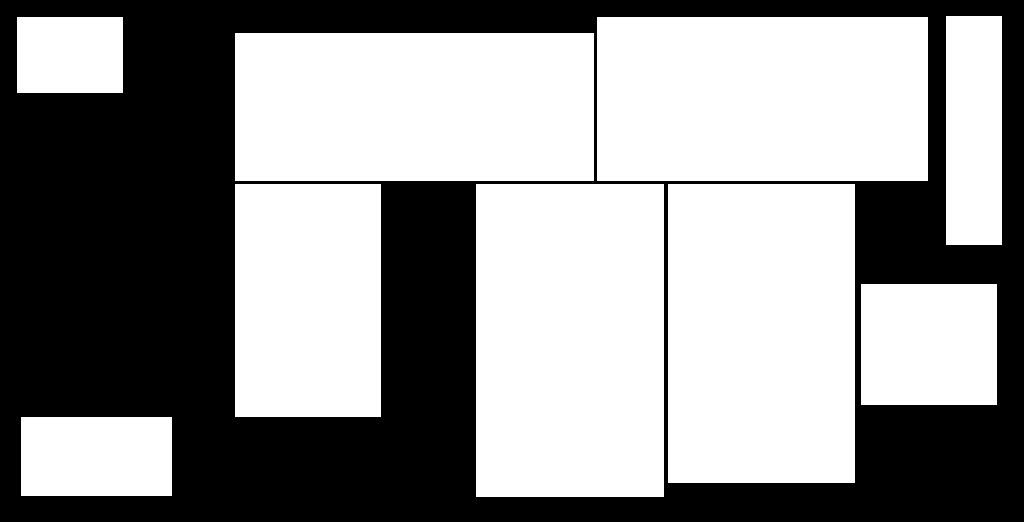
\includegraphics[width=.33\textwidth]{notes-masks/500eu-front-mask}\\
		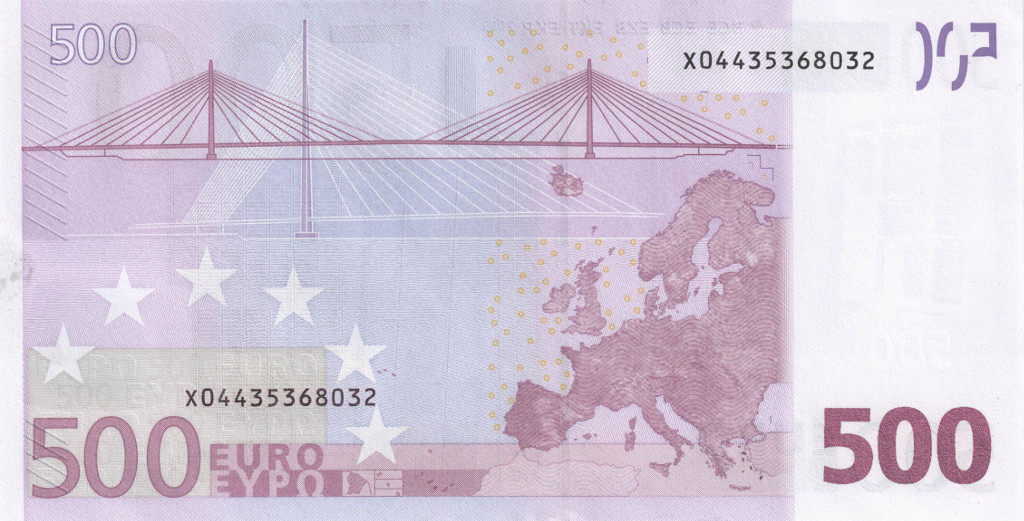
\includegraphics[width=.33\textwidth]{notes-masks/500eu-back}
		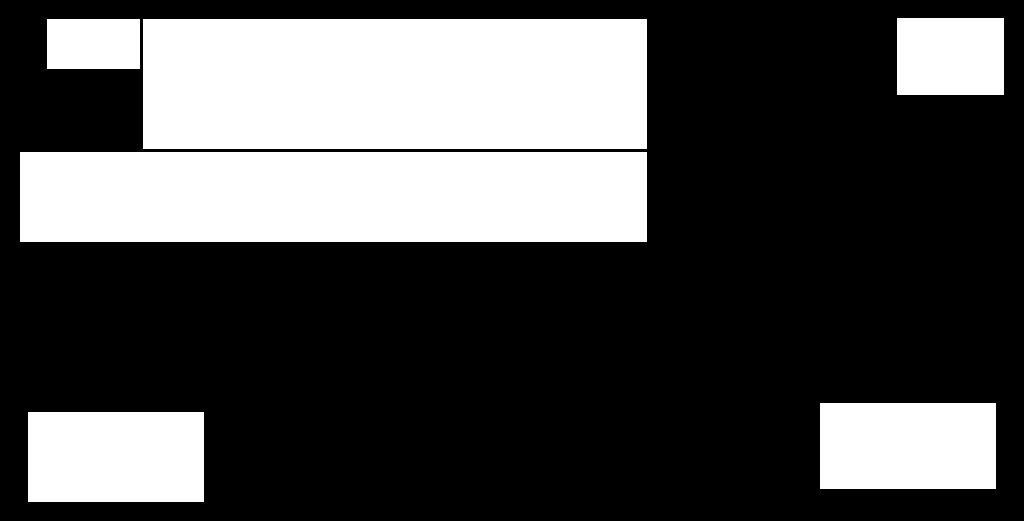
\includegraphics[width=.33\textwidth]{notes-masks/500eu-back-mask}
		\caption{Front and back of a 500\,\euro{} banknote with associated feature detection masks}
		\label{fig:banknote-feature-detection-mask-500-front}
	\end{figure}
\end{frame}


\subsection{Image Preprocessing}
\begin{frame}{Image Preprocessing}
	\begin{itemize}
		\item Bilateral filter
		\item Contrast Limited Adaptive Histogram Equalization
		\item Contrast and brightness tunning
	\end{itemize}
	
	\begin{figure}[H]
		\centering
		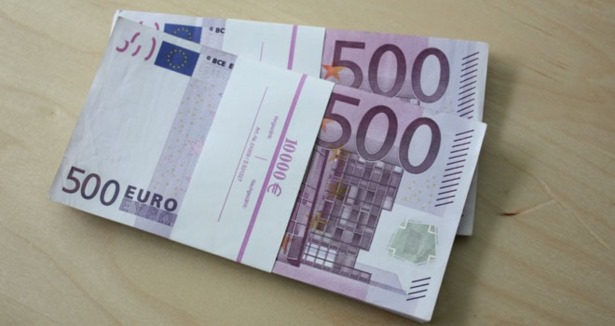
\includegraphics[width=.4\textwidth]{preprocessing/500-500}
		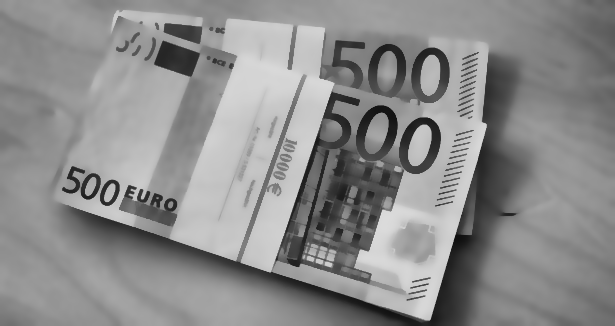
\includegraphics[width=.4\textwidth]{preprocessing/500-500-preprocessed}\\
		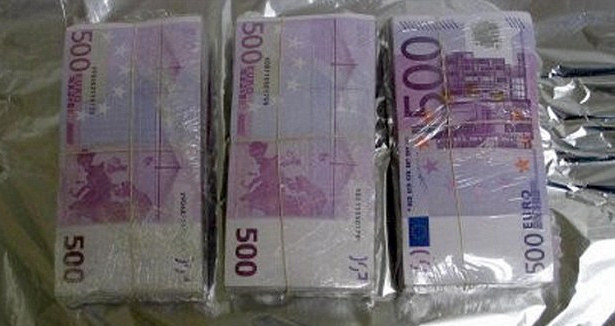
\includegraphics[width=.4\textwidth]{preprocessing/500-500-500}
		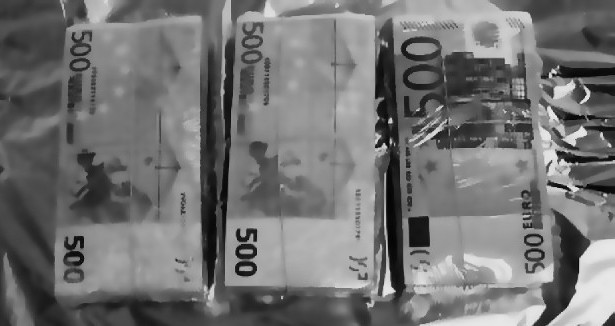
\includegraphics[width=.4\textwidth]{preprocessing/500-500-500-preprocessed}
		\caption{Impact of preprocessing stage on two pairs of images (original image on the left, preprocessed image on the right)}
		\label{fig:preprocessing}
	\end{figure}
\end{frame}


\subsection{Image Analysis}
\begin{frame}{Image Analysis}
	\begin{itemize}
		\item Keypoint detection
		\begin{itemize}
			\item SIFT, SURF, GFTT, FAST, ORB, BRISK, STAR, MSER
		\end{itemize}
		\item Keypoint description
		\begin{itemize}
			\item SIFT, SURF, FREAK, BRIEF, ORB, BRISK
		\end{itemize}
	\end{itemize}
	
	\begin{figure}[H]
		\centering
		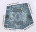
\includegraphics[width=.2496\textwidth]{image-resolution/500eu-front-very-low}\hfill
		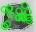
\includegraphics[width=.2496\textwidth]{image-resolution/500eu_front_currencyDB_veryLowResolution_SIFT-Detector}\hfill
		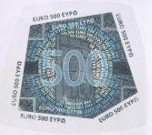
\includegraphics[width=.2499\textwidth]{image-resolution/500eu-front-medium}\hfill
		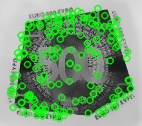
\includegraphics[width=.2499\textwidth]{image-resolution/500eu_front_currencyDB_mediumResolution_SIFT-Detector}
		\caption{Impact of image resolution when computing SIFT keypoints from a very low resolution image (left) to a high resolution image (right) of the hologram of a 500\,\euro{} banknote}
		\label{fig:banknote-500-front-resolution-difference}
	\end{figure}
\end{frame}


\subsection{Banknote Recognition}
\begin{frame}{Banknote Recognition}
	\begin{itemize}
		\item Keypoint feature matching
		\begin{itemize}
			\item Brute Force Matcher, FLANN Matcher
		\end{itemize}
	\end{itemize}

	\begin{figure}[H]
		\centering
		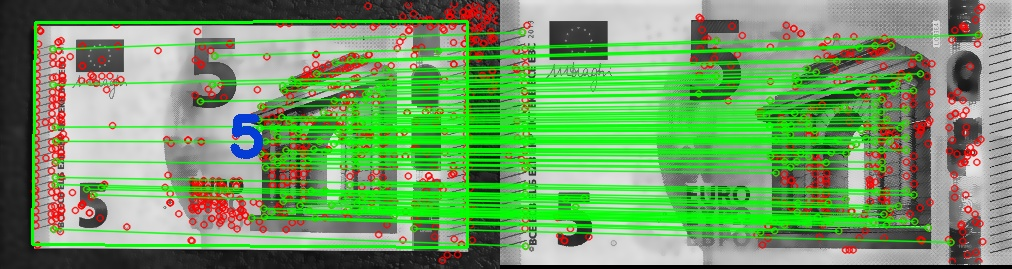
\includegraphics[width=\textwidth]{notes-recognition/5__(5).jpg___SIFT-Detector_SIFT-Extractor_BF-Matcher_lowQualityImageDB_globalMatch__inliersMatches__0}
		\caption{Feature matching on a banknote in an ideal perspective view (using SIFT detector, SIFT descriptors and BFMatcher)}
		\label{fig:recognition-front}
	\end{figure}
\end{frame}


\subsection{Recognition Analysis}
\begin{frame}{Recognition Analysis}
	\begin{itemize}
		\item Recognition inliers filtering using
		\begin{itemize}
			\item Matched descriptors ratio test
			\item Homography computed with RANSAC
		\end{itemize}
		
		\item Banknote contour with
		\begin{itemize}
			\item Reasonable area
			\item Convex shape
		\end{itemize}
		
		\item Within acceptable ranges
		\begin{itemize}
			\item Circularity
			\item Aspect ratio
			\item Global and local (mask patch) inliers percentage
		\end{itemize}
	\end{itemize}

	\begin{figure}
		\centering
		
\includegraphics[width=0.35\textwidth]{notes-masks/currency-db-shapes}
		\caption{Database of valid instances of banknote shapes}
		\label{fig:currency-db-shapes}
	\end{figure}
\end{frame}


\subsection{Recognition Output Overlay}
\begin{frame}{Recognition Output Overlay}
	\begin{itemize}
		\item If recognition successful, matched inliers are removed and the system tries to recognize another banknote
		\item Otherwise it is created an image overlay with the recognized banknotes contours and values
	\end{itemize}
	\begin{figure}[H]
		\centering
		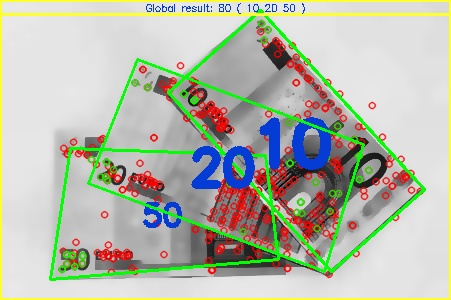
\includegraphics[width=0.6\textwidth]{notes-recognition/10-20-50.jpg___SIFT-Detector_SIFT-Extractor_BF-Matcher_dynamicQualityImageDB_globalMatch}
		\caption{Image overlay containing the recognized banknotes values and contours (used SIFT detector, SIFT descriptors and BFMatcher)}
		\label{fig:recognition-overlapping-banknotes-0}
	\end{figure}
\end{frame}

\section{\scshape Testing Dataset}\label{sec:testing-dataset}

\subsection*{Dataset Overview}
\begin{frame}{Dataset Overview}
	\begin{table}[ht]
		\centering
		\caption{Testing dataset overview (80 banknotes)}
		\small
		\begin{tabu} to 0.9\textwidth { X[2.7,l,m] X[l,m] X[l,m] X[l,m] X[l,m] X[l,m] X[l,m] X[l,m] }
			\textbf{Banknote value} & 5\,\euro{} & 10\,\euro{} & 20\,\euro{} & 50\,\euro{} & 100\,\euro{} & 200\,\euro{} & 500\,\euro{}	\\
			\noalign{\vskip 2mm} 
			\hline
			\noalign{\vskip 2mm} 
			\textbf{Nº of banknotes}			& 15		 & 12		   & 19			 & 19		   & 6			  & 9			 & 15			\\
		\end{tabu}
		\label{tab:dataset-overview}
	\end{table}

	\begin{table}[ht]
		\caption{Number of banknotes per image}
		\centering
		\small
		\begin{tabu} { X[c,m] X[c,m] X[c,m] }
			\rowfont{\bfseries\itshape} Images with 1 banknote & Images with 2 banknotes & Images with 3 banknotes \\
			\noalign{\vskip 2mm} 
			\hline
			\noalign{\vskip 2mm} 
			67			   & 11				  & 2	\\
		\end{tabu}
		\label{tab:number-of-banknotes-per-image}
	\end{table}
\end{frame}

\section{\scshape Results}\label{sec:results}

\subsection*{Results Overview}
\begin{frame}{Results Overview}
	\begin{table}[ht]
		\caption{Selection of the configurations with the best recognition results (1 configuration per image)}
		\centering
		\small
		\begin{tabu} { X[0.6,c,m] X[0.8,c,m] X[c,m] X[c,m] X[c,m] }
			\rowfont{\bfseries\itshape} Detector & Descriptor & Images with 1 banknote & Images with 2 banknotes & Images with 3 banknotes \\
			\noalign{\vskip 2mm} 
			\hline
			\noalign{\vskip 2mm} 
			SIFT	 & SIFT		  & 37			   & 7				  & 2	\\
			SURF	 & SURF		  & 24			   & 3				  & 0	\\
			GFTT	 & SIFT		  & 3			   & 1				  & 0	\\
			FAST	 & SIFT		  & 1			   & 0				  & 0	\\
			BRISK	 & BRISK	  & 1			   & 0				  & 0	\\
			ORB		 & ORB		  & 1			   & 0				  & 0	\\
		\end{tabu}
		\label{tab:recognition-configurations}
	\end{table}
\end{frame}


\subsection*{Front View Recognition With Clutter}
\begin{frame}{Front View Recognition With Clutter}
		\begin{figure}[H]
			\centering
			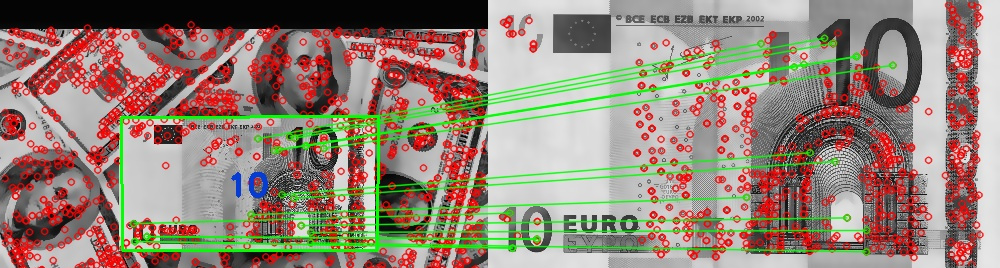
\includegraphics[width=\textwidth]{notes-recognition/10__(9).jpeg___SIFT-Detector_SIFT-Extractor_BF-Matcher_lowQualityImageDB_globalMatch__inliersMatches__0}
			\caption{Detection of a banknote in an ideal perspective view with background clutter (using SIFT detector, SIFT descriptors and BFMatcher)}
			\label{fig:recognition-clutter}
		\end{figure}
\end{frame}


\subsection*{Recognition With Perspective Distortion}
\begin{frame}{Recognition With Perspective Distortion}
	\begin{figure}[H]
		\centering
		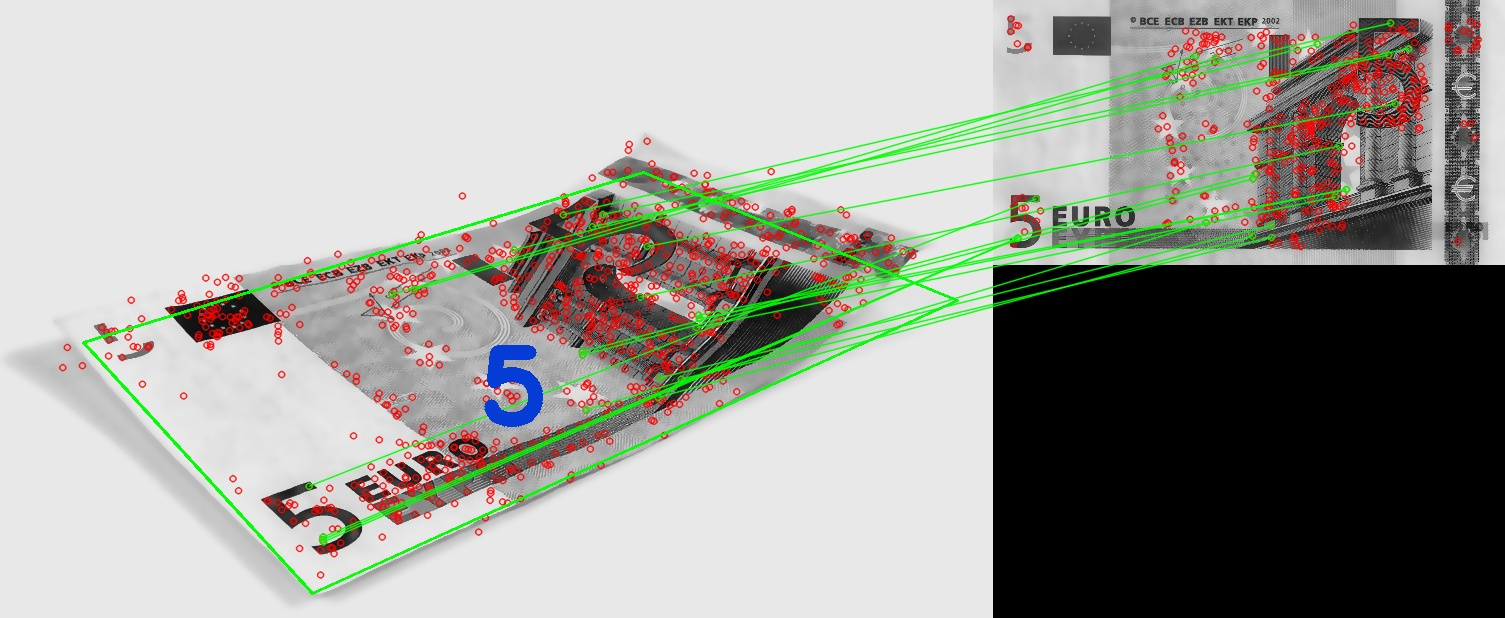
\includegraphics[width=\textwidth]{notes-recognition/5__(6).jpg___SURF-Detector_SURF-Extractor_BF-Matcher_lowQualityImageDB_globalMatch__inliersMatches__0}
		\caption{Detection of banknotes with perspective distortion and folding (using SURF detector, SURF descriptors and BFMatcher)}
		\label{fig:recognition-perspective-distortion}
	\end{figure}
\end{frame}


\subsection*{Recognition With Folding}
\begin{frame}{Recognition With Partial Folding}
	\begin{figure}[H]
		\centering
		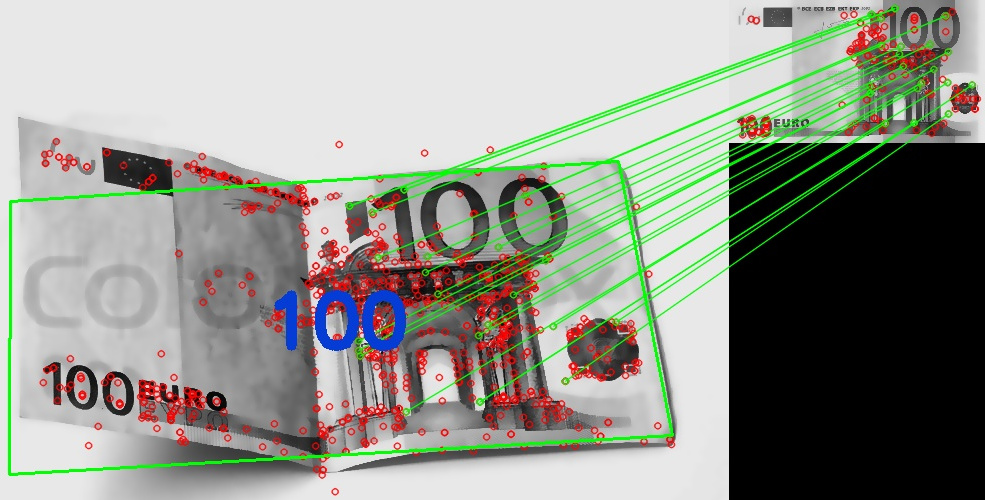
\includegraphics[width=\textwidth]{notes-recognition/100__(4).jpg___SIFT-Detector_SIFT-Extractor_BF-Matcher_dynamicQualityImageDB_globalMatch__inliersMatches__0.jpg}
		\caption{Detection of partially folded banknotes\\(using SIFT detector, SIFT descriptors and BFMatcher)}
		\label{fig:recognition-folding}
	\end{figure}
\end{frame}


\subsection*{Recognition With Occlusion}
\begin{frame}{Recognition With Occlusion}
	\begin{figure}[H]
		\centering
		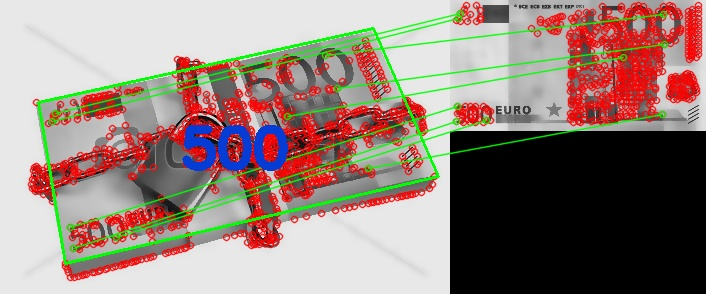
\includegraphics[width=\textwidth]{notes-recognition/500.jpg___GFTT-Detector_SIFT-Extractor_BF-Matcher_dynamicQualityImageDB_globalMatch__inliersMatches__0}
		\caption{Detection of partially occluded banknotes\\(using GFTT detector, SIFT descriptors and BFMatcher)}
		\label{fig:recognition-partially-occluded-banknotes}
	\end{figure}
\end{frame}


\subsection*{Recognition Of Partially Visible Banknotes}
\begin{frame}{Recognition Of Partially Visible Banknotes}
	\begin{figure}[H]
		\centering
		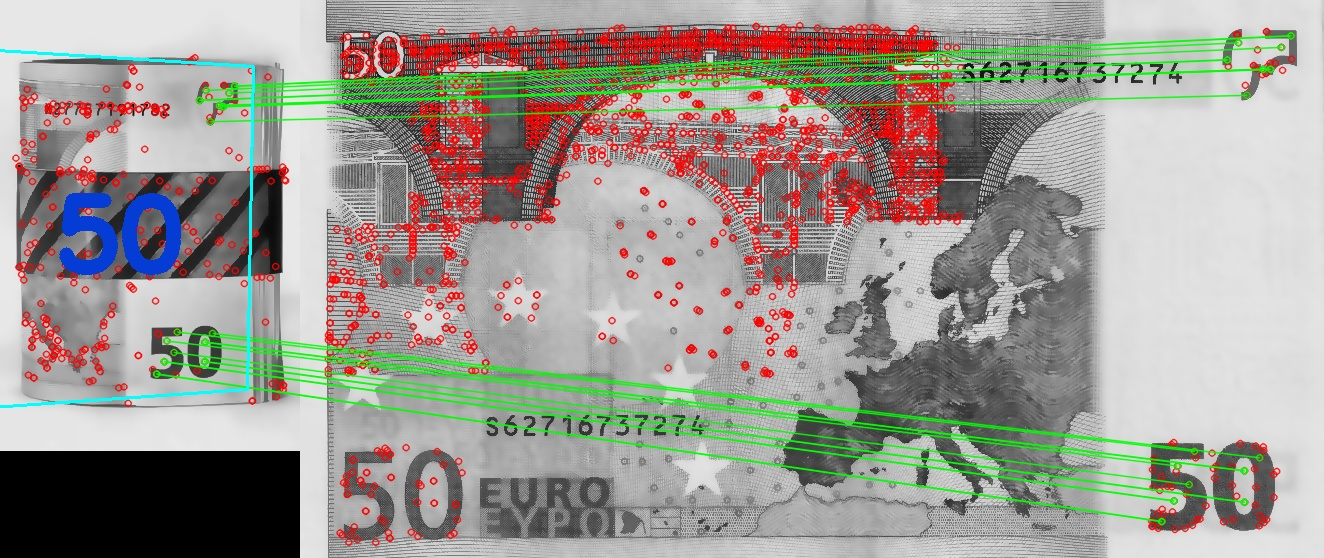
\includegraphics[width=\textwidth]{notes-recognition/50__(13).jpg___SIFT-Detector_SIFT-Extractor_BF-Matcher_mediumQualityImageDB_globalMatch__inliersMatches__0}
		\caption{Detection of partially visible banknotes\\(using SIFT detector, SIFT descriptors and BFMatcher)}
		\label{fig:recognition-partially-visible}
	\end{figure}
\end{frame}


\subsection*{Recognition Of Multiple Banknotes}
\begin{frame}{Recognition Of Multiple Banknotes}
	\begin{figure}[H]
		\centering
		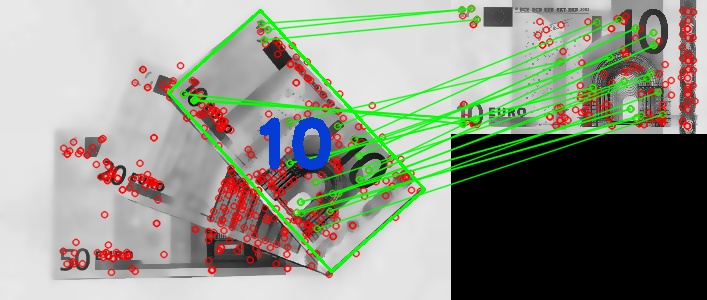
\includegraphics[width=\textwidth]{notes-recognition/10-20-50.jpg___SIFT-Detector_SIFT-Extractor_BF-Matcher_dynamicQualityImageDB_globalMatch__inliersMatches__1}
		\caption{Detection of overlapping banknotes\\(using SIFT detector, SIFT descriptors and BFMatcher)}
		\label{fig:recognition-overlapping-banknotes-1}
	\end{figure}
\end{frame}

\subsection*{Recognition Of Multiple Banknotes}
\begin{frame}{Recognition Of Multiple Banknotes}
	\begin{figure}[H]
		\centering
		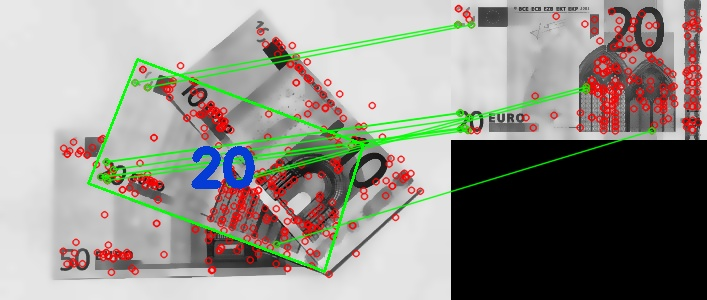
\includegraphics[width=\textwidth]{notes-recognition/10-20-50.jpg___SIFT-Detector_SIFT-Extractor_BF-Matcher_dynamicQualityImageDB_globalMatch__inliersMatches__2}
		\caption{Detection of overlapping banknotes\\(using SIFT detector, SIFT descriptors and BFMatcher)}
		\label{fig:recognition-overlapping-banknotes-2}
	\end{figure}
\end{frame}

\subsection*{Recognition Of Multiple Banknotes}
\begin{frame}{Recognition Of Multiple Banknotes}
	\begin{figure}[H]
		\centering
		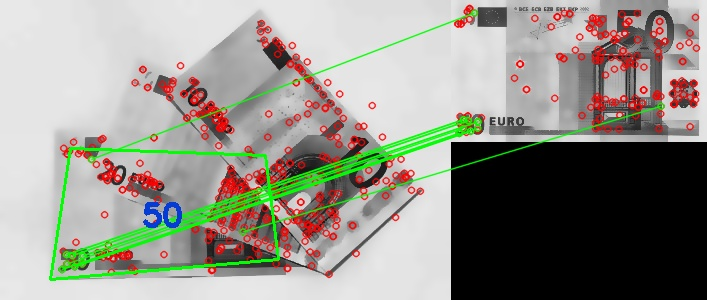
\includegraphics[width=\textwidth]{notes-recognition/10-20-50.jpg___SIFT-Detector_SIFT-Extractor_BF-Matcher_dynamicQualityImageDB_globalMatch__inliersMatches__0}
		\caption{Detection of overlapping banknotes\\(using SIFT detector, SIFT descriptors and BFMatcher)}
		\label{fig:recognition-overlapping-banknotes-3}
	\end{figure}
\end{frame}



\section{\scshape Summary}\label{sec:summary}

\begin{frame}{Summary}
	Text.
\end{frame}



\end{document}
